\chapter{Previous Work}

Many research have been done in stylizing 3D scene\cite{schmid_overcoat:_2011, praun_real-time_2001, klein_non-photorealistic_2000, benard_dynamic_2009, benard_dynamic_2010, freudenberg_walk-through_2001, benard_state---art_2011} trying to propose solutions or trade-offs for the problem of \textit{temporal coherence}. In this part of this report, we will present you techniques to stylize 3D scenes and we will show their advantages and disadvantages. In order to render an image of a 3D object in the screen, a graphics program goes through several steps that compute some different information like the gradient of the image, the shadows made by the object, the amount of light received by the object, etc. The gathering of all these steps is called \textbf{graphical pipeline rendering}. In this graphical pipeline, there are two moments when we can stylize the objects. The first is when we computed information about the geometry of each object in the scene, we call it \textit{object space}. The second moment is when we gather the previously computed images of the scene in order to make for example shadows, global illumination, ambient occlusion, etc. we call it the \textit{image space}. We will treat these two space separately and with the two different types of methods to stylize.



\section{Object Space}


\begin{figure}
    \begin{center}
    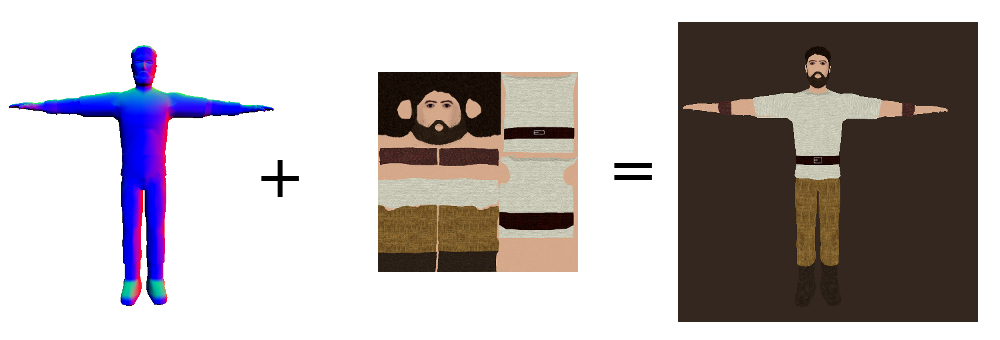
\includegraphics[scale=0.2]{pics/texture_mapping.png}
    \end{center}
    \caption{Texture mapping: example}
    \label{texture_mapping}
\end{figure}

\begin{figure}
    \begin{center}
    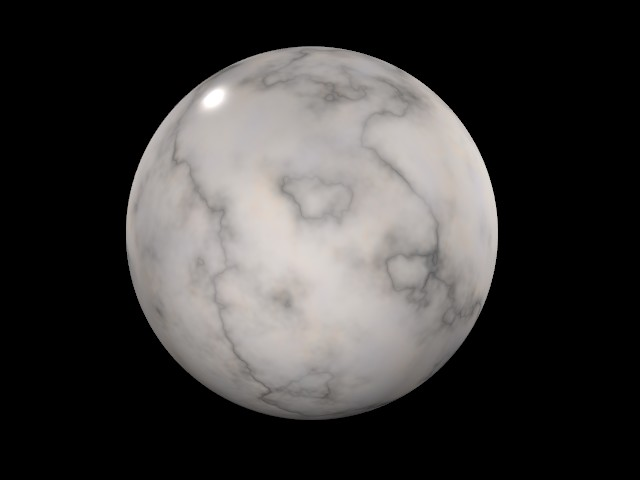
\includegraphics[scale=0.2]{images/marble.jpg}
    \end{center}
    \caption{Marble with procedural texture}
    \label{marble_rendering}
\end{figure}





In the object space, we work on the surface of the object and so we have all the knowledge about the geometry. \newline

% texture based

\textbf{Texture-based methods}

One of the most used ways to colored object in 3D is the \textit{texture mapping}. It consists of mapping an image on the object \ref{texture_mapping}. This technique is widely used in video games because it is easy to implement, it can be implemented for GPU and it needs low computation. As shown in the example, texture mapping can be used with images as a texture in order to stylize the object\cite{praun_real-time_2001, klein_non-photorealistic_2000, freudenberg_walk-through_2001}. Texture mapping can also be done with \textit{procedural noises}\cite{perlin_improving_2002} in this case called \textit{procedural textures}. Procedural textures are mathematically computed from coordinates the most famous is Perlin but there exist others like Gabor noise, Worley noise, etc. With these textures, we can create images looks like marble \ref{marble_rendering} or realist wood. Bénard et al.\cite{benard_dynamic_2009, benard_dynamic_2010} use this method of texture mapping with noise in order to make watercolor stylization. \newline

This method has a problem of \textit{foreshortening} of the silhouettes which makes an area with more elements than in the center of the object and when zooming in/out the size of the elements in the mapped texture vary depending on the distance from the camera, if we get closer to the object the elements on the texture become bigger and bigger going up to pixelization sometimes. These two problems make texture mapping bad in term of \textit{flatness} because an artist does not draw bigger strokes if the object is close and does not draw more details at the silhouettes than in the center of his objects. Texture mapping is also bad in term of variety of style that you can do because you are depending on the texture chosen you cannot, for instance, do a rendered image that looks like painted with brushes and especially you cannot change the shape of the object in the rendered image, a perfect sphere will always appear as a perfect sphere. On the other hand, this method naturally ensures \textit{motion coherence} and \textit{temporal continuity} because the texture is mapped directly on the surface of the object. \newline





\textbf{Mark based methods}

The natural way to stylize 3D objects is to as an artist apply paint strokes on the object. These paint strokes can be represented with smalls images also called splats. Daniels\cite{Daniels_1999} and Schmid\cite{schmid_overcoat:_2011} propose to project splats composed of stroke and stored them on the geometry of the model but this technique is expensive in term of storage. Some works \cite{meier_painterly_1996, Fekete_2000, chi_stylized_2006}(more in the state of the art \cite{benard_state---art_2011}) use point distribution in order to make anchor points for splats. These point distributions are often computed in image space and then are projected on the model. Anchor these splats to the model improve the \textit{motion coherence} because each splat will follow the motion of the 3D model. These splats are rendered in the image space as a 2D sprites so preserved the \textit{flatness}. The problem is how to have the point distribution and how can we control it in order to have a uniform, not too sparse and not too dense distribution. Moreover, these point distribution does not provide control over the \textit{temporal continuity}. In our method, we use procedural noise to anchor the splats.


\section{Image space}

\textbf{Texture-based methods}

Many methods to stylize in image space used texture based approaches. It consists to apply the texture to the entire image \cite{benard_state---art_2011} but in the case of stylizing animated scenes, the problem is how do we deform the texture to minimize the apparition of sliding artefacts. We can distinguish two families of approaches to solve this problem. The first family of approaches use an approximation of the 3D camera motion with 2D transformations of the texture\cite{cunzi_dynamic_nodate}. This gives a nice trade-off between \textit{motion coherence} and \textit{flatness} but it is limited to static scenes and a set of few camera motions. Moreover, sliding artefacts still occur with strong parallax so Fung et al.\cite{fung_pen-and-ink_nodate} and Breslav et al.\cite{breslav_dynamic_nodate} improve the approximation of the scene motion in order to reduce sliding artefacts.

The second family of approaches use non-rigid deformations to animate the texture\cite{bousseau_video_2007}. These deformations are computed from the optical flow of a video. This is an extension of the methods used in vector field visualization by Neyret\cite{neyret_imagis-gravir_nodate}. These deformations can distort the texture and alter the original pattern. The method of Bousseau et al.\cite{bousseau_video_2007} is very effective with stochastic textures as the fractalization process but creates artefacts with structured patterns. \newline



\textbf{Mark based methods}

A method very used to stylize in image space consists to draw strokes/splats at some place of the image\cite{bleron_motion-coherent_2018, vergne_implicit_2011, benard_active_nodate, zeng_image_2009, grabli_programmable_2010}. The question of these mark based method is where do we place the marks in order to have a stylized rendering without losing the meaning of the scene. A first approach is to extract lines that are relevant like the silhouettes, etc. \cite{vergne_implicit_2011, grabli_programmable_2010, lee_line_nodate} and then stylize the image with this information, like keeping only the extracted lines and change the shape of each line or apply strokes along these lines as Vergne et al.\cite{vergne_implicit_2011} did try to have a good \textit{temporal coherence}. The problem of these techniques is the popping marks due to a bad \textit{temporal continuity}.
A second approach is to segment the image in order to have the different parts of the scene\cite{zeng_image_2009, lin_video_nodate}. Thanks to this segmentation, they apply different strokes for each part of the image with the corresponding colors. The work of Lin et al.\cite{lin_video_nodate} is about videos so they use the optical flow of the videos in order to have a good \textit{temporal coherence}. These mark based methods have a good impression of \textit{flatness} thanks to the splatting in image space, this is something that we will use in our approach.


\begin{figure}

    \begin{tabular}{|l|*{4}{c|}}
    \hline
         & \textbf{Motion coherence} & \textbf{Flatness} & \textbf{Temporal continuity} & \textbf{Style variation} \\
    \hline
    \textbf{Object space} & & & & \\
    \hline
    Texture-based methods & ++ & - - & ++ & - - \\
    \hline
    Mark based methods & ++ & + & - & +/- \\
    \hline
    \textbf{Image space} & & & & \\
    \hline
    Texture-based methods & -  & ++ & + & - - \\
    \hline
    Mark based methods & - & ++ & - - & + \\
    \hline
    \end{tabular}

    \caption{Summary of trade-offs made in different approaches}
    \label{tableau_comparatif}
\end{figure}
